%------------------------------------------------------------------------------%
%        1         2         3         4         5         6         7         %
% 3456789 123456789 123456789 123456789 123456789 123456789 123456789 12345678 %
%        0         0         0         0         0         0         0         %
%------------------------------------------------------------------------------%
%
% Cameron Crowe
% trailsangha@gmail.com
% http://www.trailsangha.com
% http://www.github.com/trailsangha/omz-sutrabook
%
% Ordinary Mind Zendo sutrabook
%
% MIT License
% 
% Copyright (c) 2022 Ordinary Mind Zendo
% 
% Permission is hereby granted, free of charge, to any person obtaining a copy
% of this software and associated documentation files (the "Software"), to deal
% in the Software without restriction, including without limitation the rights
% to use, copy, modify, merge, publish, distribute, sublicense, and/or sell
% copies of the Software, and to permit persons to whom the Software is
% furnished to do so, subject to the following conditions:
% 
% The above copyright notice and this permission notice shall be included in all
% copies or substantial portions of the Software.
% 
% THE SOFTWARE IS PROVIDED "AS IS", WITHOUT WARRANTY OF ANY KIND, EXPRESS OR
% IMPLIED, INCLUDING BUT NOT LIMITED TO THE WARRANTIES OF MERCHANTABILITY,
% FITNESS FOR A PARTICULAR PURPOSE AND NONINFRINGEMENT. IN NO EVENT SHALL THE
% AUTHORS OR COPYRIGHT HOLDERS BE LIABLE FOR ANY CLAIM, DAMAGES OR OTHER
% LIABILITY, WHETHER IN AN ACTION OF CONTRACT, TORT OR OTHERWISE, ARISING FROM,
% OUT OF OR IN CONNECTION WITH THE SOFTWARE OR THE USE OR OTHER DEALINGS IN THE
% SOFTWARE.
%

\documentclass[12pt]{report}

%%%%%%% GEOMETRY

\usepackage[paper=letterpaper, margin=1in]{geometry}

%%%%%%% FONTS

% Encoding
\usepackage[T1]{fontenc}          % Extent font encoding
\usepackage[utf8]{inputenc}       % Utf8 character encoding

% Default
\linespread{1.1}                  % Scale line spacing
\usepackage[default]{gillius}     % Gillius!!!

% Japanese
\newcommand{\sbJapanese}[1]{
  \newdimen\origiwspc
  \origiwspc=\fontdimen2\font
  \fontdimen2\font=1.2ex
  {#1}
  \fontdimen2\font=\origiwspc
}


%%%%%%% TABLE OF CONTENTS

\usepackage[linktocpage=true]{hyperref} % Hyperlinks in toc.

%%%%%%% SECTIONING

\newcommand{\sbSection}[1]{
  \section*{#1}
  \addcontentsline{toc}{section}{#1}
}

%%%%%%% GRAPHICS

\usepackage{graphicx}        % Include images
\graphicspath{ {./images/} } % Image directory

%%%%%%% COLUMNS

\usepackage{multicol}             % http://ctan.org/pkg/multicol
\setlength{\parindent}{0pt}       % Pragraph indent (in multicol environment)


%------------------------------------------------------------------------------%
%        1         2         3         4         5         6         7         %
% 3456789 123456789 123456789 123456789 123456789 123456789 123456789 12345678 %
%        0         0         0         0         0         0         0         %
%------------------------------------------------------------------------------%

\begin{document}

% Title Page
% ==========

\begin{titlepage}
	\centering
  \null
	\vfill
  {\huge Ordinary Mind Zendo\par}
  \vspace{0.25in}
  {\Huge Sutra Book\par}
	\vfill
	{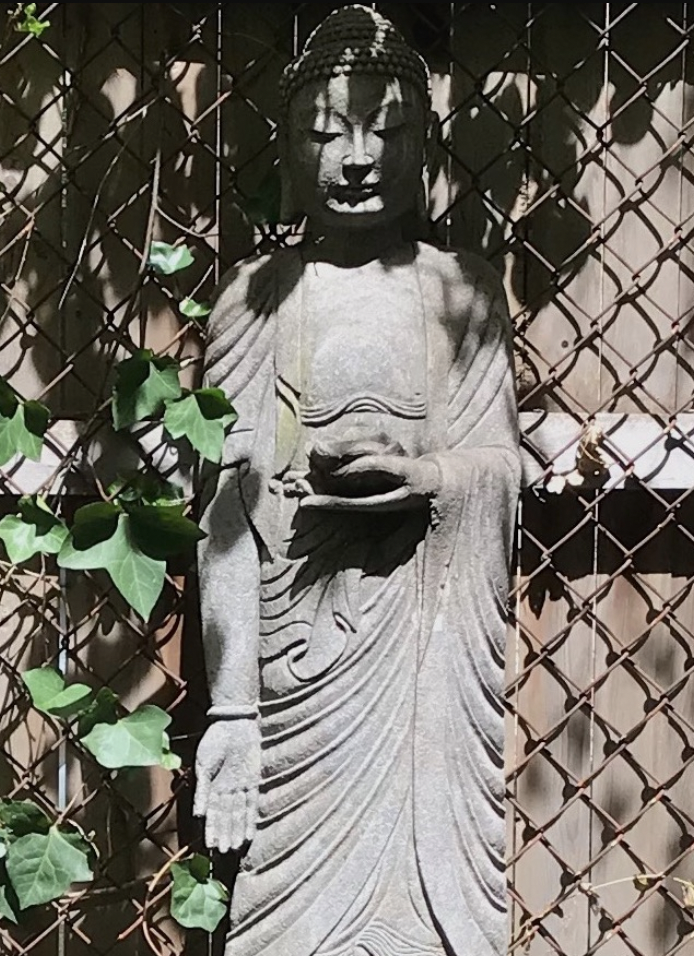
\includegraphics[width=0.30\textwidth]{omz-garden-statue.png}\par}
	\vfill
  {\large \emph{Buddha Nature is impermanence.}\par}
	\vfill
	{\large \today\par}

% Bottom of the page
\end{titlepage}


\newpage 

% Table of Contents
% =================

\renewcommand{\vspace}[2]{} % Remove extra space above table of contents
\tableofcontents

\newpage 

\sbSection{Maha Prajna Paramita Heart Sutra}
% ==========================================

Avalokitesvara Bodhisattva, doing deep prajna paramita,\\
Clearly saw emptiness of all the five conditions,\\
Thus completely relieving misfortune and pain.\\
O Shariputra, Form is no other than emptiness,\\
Emptiness no other than form;\\
Form is exactly emptiness, emptiness exactly form;\\
Sensation, conception, discrimination, awareness\\
Are likewise like this.\\
O Shariputra, all dharmas are forms of emptiness,\\
Not born, not destroyed\\
Not stained, not pure,\\
Without loss, without gain;\\
So in emptiness there is no form, no sensation, conception,\\
discrimination, awareness;\\
No eye, ear, nose, tongue, body, mind;\\
No color, sound, smell, taste, touch, phenomena;\\
No realm of sight, no realm of consciousness;\\
No ignorance and no end to ignorance;\\
No old age and death, and no end to old age and death;\\
No suffering, no cause of suffering;\\
No extinguishing, no path; no wisdom and no gain.\\
No gain and thus the Bodhisattva lives prajna paramita\\
With no hindrance in the mind;\\
No hindrance, therefore no fear.\\
Far beyond deluded thoughts, this is nirvana.\\
All past, present and future buddhas live prajna paramita,\\
And therefore attain anutara-samyak-sambodhi.\\
Therefore know prajna paramita is\\
The great mantra, the vivid mantra,\\
The best mantra, the unsurpassable mantra;\\
It completely clears all pain -- this is the truth not a lie.\\
So set forth the prajna paramita mantra,\\
Set forth this mantra and say:\\
Gate! Gate! Paragate! Parasamgate!\\
Bodhi svaha! Prajna heart sutra!

\newpage 

\sbSection{Maka Hannya Haramita Shin Gyo}
% =======================================

\sbJapanese{
  %MAKA HANNYA HARAMITA SHIN GYO\\
  KAN JI ZAI BO SA GYO JIN HAN NYA HA RA MI\\
  TA JI SHO KEN GO ON KAI KU DO IS SAI KU\\
  YAKU SHA RI SHI SHIKI FU I KU KU FU I SHIKI\\
  SHIKI SOKU ZE KU KU SOKU ZE SHIKI JU SO GYO SHIKI\\
  YAKU BU NYO ZE SHA RI SHI ZE SHO HO KU SO\\
  FU SHO FU METSU FU KU FU JO FU ZO FU GEN\\
  ZE KO KU CHU MU SHIKI MU JU SO GYO SHIKI MU\\
  GEN NI BI ZES SHIN NI MU SHIKI SHO KO MI SOKU\\
  HO MU GEN KAI NAI SHI MU I SHIKI KAI MU MU\\
  MYO YAKU MU MU MYO JIN NAI SHI MU RO SHI YAKU\\
  MU RO SHI JIN MU KU SHU METSU DO MU CHI YAKU\\
  MU TOKU I MU SHO TOK KO BO DAI SAT TA E\\
  HAN NYA HA RA MI TA KO SHIN MU KE GE MU\\
  KE GE KO MU U KU FU ON RI IS SAI TEN\\
  DO MU SO KU GYO NE HAN SAN ZE SHO BUTSU E\\
  HAN NYA HA RA MI TA KO TOKU A NOKU TA RA\\
  SAM MYAKU SAM BO DAI KO CHI HAN NYA HA RA MI\\
  TA ZE DAI JIN SHU ZE DAI MYO SHU ZE MU JO\\
  SHU ZE MU TO TO SHU NO JO IS SAI KU SHIN\\
  JITSU FU KO KO SETSU HAN NYA HA RA MI TA SHU\\
  SOKU SETSU SHU WATSU GYA TEI GYA TEI HA RA GYA TEI\\
  HARA SO GYA TEI BO JI SOWA KA HAN NYA SHIN GYO
}

\newpage 

\sbSection{Identity of Relative and Absolute}
% ===========================================

The mind of the Great Sage of India was intimately conveyed from west to east.\\
Among human beings are wise ones and fools.\\
But in the way there is no northern or southern ancestor.\\
The subtle source is clear and bright;\\
The tributary streams flow through the darkness.\\
To be attached to things is illusion;\\
To encounter the absolute is not yet enlightenment.\\
Each and all, the subjective and objective spheres are related,\\
And at the same time independent.\\
Related, yet working differently, though each keeps its own place.\\
Form makes the character and appearance different;\\
Sounds distinguish comfort and discomfort.\\
The dark makes all words one;\\
The brightness distinguishes good and bad phrases.\\
The four elements return to their nature as a child to its mother.\\
Fire is hot, wind moves, water is wet, earth hard.\\
Eyes see, ears hear, nose smells, tongue tastes the salt and sour\\
Each is independent of the other;\\
Cause and effect must return to the great reality.\\
The words high and low are used relatively.\\
Within light there is darkness,\\
But do not try to understand that darkness;\\
Within darkness there is light,\\
But do not look for that light.\\
Light and darkness are a pair,\\
Like the foot before and the foot behind, in walking.\\
Each thing has its own intrinsic value and is\\
Related to everything else in function and position.\\
Ordinary life fits the absolute as a box and its lid.\\
The absolute works together with the relative\\
Like two arrows meeting in mid-air.\\
Reading words you should grasp the great reality.\\
Do not judge by any standards.\\
If you do not see the way, you do not see it\\
even as you walk on it.\\
When you walk the way, it is not near, it is not far.\\
If you are deluded, you are mountains and rivers away from it.\\
I respectfully say to those who wish to be awakened:\\
Do not waste your time by night or day.

\newpage 

\sbSection{Sandokai}
% ==================

\sbJapanese{
  CHI KU DO DAI SEN NO SHIN TO ZAI MITSU NI AI\\
  FU SU NIN KON NI RI DON ARI DO NI NAM BO\\
  KU NO SO NASHI REI GEN MYO NI KO KET TARI SHI\\
  HA AN NI RU CHU SU JI WO SHU SU RU MO\\
  MOTO KO RE MA YOI RI NI KA NO MO MATA SA\\
  TO RI NI ARA ZU MON MON IS SAI NO KYO EGO\\
  TO FU EGO TO E SHI TE SA RA NI AI WATA\\
  RU SHI KARA ZA RE BA KU RAI NI YO TE JU\\
  SU SHIKI MOTO SHITSU ZO WO KO TO NI SHI SHO MOTO\\
  RAK KU WO KO TO NI SU AN WA JO CHU NO\\
  KOTO NI KA NAI MEI WA SEI DAKU NO KU WO WA\\
  KA TSU SHI DAI NO SHO ONO ZU KARA FU KU SU\\
  KO NO SONO HA HA WO URU GA GO TO SHI HI\\
  WA NES SHI KA ZE WA DO YO MI ZU WA URU\\
  OI CHI WA KEN GO MA NA KO WA IRO MIMI WA\\
  ON JO HANA WA KA SHI TA WA KAN SO SHI KA\\
  MO ICHI ICHI NO HO NI OI TE NE NI YO TE\\
  HA BUM PU SU HO MATSU SU BE KARA KU SHU NI\\
  KISU BESHI SOM PI SONO GO WO MO CHI U MEI CHU\\
  NI ATA TE AN ARI AN SO WO MO TE O KOTO\\
  NA KA RE AN CHU NI ATA TE MEI ARI MEI SO\\
  WO MO TE MI RU KO TO NA KA RE MEI AN\\
  ONO ONO AI TAI SHI TE HI SU RU NI ZEN GO\\
  NO AYU MI NO GO TO SHI BAM MO TSU ONO ZU\\
  KARA KO ARI MA SA NI YO TO SHO TO WO I\\
  U BESHI JI SON SU RE BA KAN GAI GAS SHI RI\\
  O ZU RE BA SEMPO SA SO KO TO WO UKE TE\\
  WA SU BE KARA KU SHU WO ESU BESHI MI ZU KARA\\
  KI KU WO RI SU RU KO TO NA KA RE SO\\
  KU MO KU DO WO ESE ZUM BA ASHI WO HA KO\\
  BU MO IZU KUN ZO MI CHI WO SHI RAN AYU MI\\
  WO SU SU MU RE BA GON NON NI ARA ZU MA\\
  YO TE SEN GA NO KO WO HE DA TSU TSU TSU\\
  SHIN DE SAN GEN NO HI TO NI MO SU KO IN\\
  MU NA SHI KU WA TA RU KO TO NA KA RE
}

\newpage 

\sbSection{The Lineage}
% =====================

\begin{multicols*}{3}    % * means let column width vary.
     Bibashi Butsu Daiosho
  \\ Shiki Butsu Daiosho 
  \\ Bishafu Butsu Daiosho
  \\ Kuruson Butsu Daiosho
  \\ Kunagommuni Butsu Daiosho
  \\ Kasho Butsu Daiosho
  \\ Shakyamuni Butsu Daiosho
  \\ Makakasho Daiosho
  \\ Ananda Daiosho
  \\ Shonawashu Daiosho
  \\ Ubakikuta Daiosho
  \\ Daitaka Daiosho
  \\ Mishaka Daiosho
  \\ Bashumitsu Daiosho
  \\ Butsudanandai Daiosho
  \\ Fudamitta Daiosho
  \\ Barishiba Daiosho
  \\ Funayasha Daiosho
  \\ Anabotei Daiosho
  \\ Kabimora Daiosho
  \\ Nagyaharajuna Daiosho
  \\ Kanadaiba Daiosho
  \\ Ragarata Daiosho
  \\ Sogyanandai Daiosho
  \\ Kayashata Daiosho
  \\ Kumorata Daiosho
  \\ Shayata Daiosho
  \\ Bashubanzu Daiosho
  \\ Manura Daiosho

  \columnbreak

     Kakurokuna Daiosho
  \\ Shishibodai Daiosho 
  \\ Bashashita Daiosho
  \\ Funyomitta Daiosho
  \\ Hannyatara Daiosho
  \\ Bodaidaruma Daiosho
  \\ Taiso Eka Daiosho
  \\ Kanchi Sosan Daiosho
  \\ Daii Doshin Daiosho
  \\ Daiman Konin Daiosho
  \\ Daikan Eno Daiosho
  \\ Seigen Gyoshi Daiosho
  \\ Sekito Kisen Daiosho
  \\ Yakusan Igen Daiosho
  \\ Ungan Donjo Daiosho
  \\ Tozan Ryokai Daiosho
  \\ Ungo Doyo Daiosho
  \\ Doan Dohi Daiosho
  \\ Doan Kanshi Daiosho
  \\ Ryozan Enkan Daiosho
  \\ Taiyo Kyogen Daiosho
  \\ Toshi Gisei Daiosho
  \\ Fuyo Dokai Daiosho
  \\ Tanka Shijun Daiosho
  \\ Choro Seiryo Daiosho
  \\ Tendo Sokaku Daiosho
  \\ Setcho Chikan Daiosho
  \\ Tendo Nyojo Daiosho
  \\ Eihei Dogen Daiosho

  \columnbreak

     Koun Ejo Daiosho
  \\ Tettsu Gikai Daiosho
  \\ Keizan Jokin Daiosho
  \\ Gasan Joseki Daiosho
  \\ Taigen Soshin Daiosho
  \\ Baizan Monpon Daiosho
  \\ Nyocho Tengin Daiosho
  \\ Kisan Shosan Daiosho
  \\ Morin Shihan Daiosho
  \\ Taishi Sotai Daiosho
  \\ Kencho Hantetsu Daiosho
  \\ Daiju Soko Daiosho
  \\ Kinpo Jusen Daiosho
  \\ Tetsuei Seiton Daiosho
  \\ Shukoku Choton Daiosho
  \\ Ketsuzan Tetsuei Daiosho
  \\ Hoshi Soon Daiosho
  \\ Goho Kainon Daiosho
  \\ Tenkei Denson Daiosho
  \\ Zozan Monko Daiosho
  \\ Niken Sekiryo Daiosho
  \\ Reitan Roryu Daiosho
  \\ Kakujo Tosai Daiosho
  \\ Kakuan Ryogu Daiosho
  \\ Ryoka Daibai Daiosho
  \\ Ungan Guhaku Daiosho
  \\ Baian Hakujun Daiosho
  \\ Hakuyu Taizan Daiosho
  \\ Joko Beck Daiosho
\end{multicols*}

\newpage 

\sbSection{Enmei Jukku Kannon Gyo}
% ================================

\sbJapanese{
  KAN ZE ON NA MU\\
  BUTSU YO\\
  BUTSU U IN YO\\
  BUTSU U EN BUP\\
  PO SO EN JO\\
  RAKU GA JO CHO NEN\\
  KAN ZE ON BO NEN\\
  KAN ZE ON NEN NEN\\
  JU SHIN KI NEN NEN\\
  FU RI SHIN
}

\sbSection{Great Vows for All}
% ============================

Sentient beings are numberless;\\
I vow to save them.\\
Delusion are inexhaustible;\\
I vow to put an end them.\\
The dharma is boundless;\\
I vow to master it.\\
The Buddha way is unsurpassable;\\
I vow to embody it.

\sbSection{Great Vows For All (Japanese)}
% =======================================

\sbJapanese{
  SHUJO MU HEN SEI GAN DO\\
  BONNO MU JIN SEI GAN DAN\\
  HO MON MU RYO SEI GAN GAKU\\
  BUTSU DO MU JO SEI GAN JO
}

\sbSection{Dedication}
% ====================

All Buddhas Throughout Space and Time,\\
All Honored Ones, Bodhisattvas, Mahasattvas,\\
Wisdom Beyond Wisdom,\\
Maha Prajna Paramita.

\end{document}

